\section{Elektrostatik}

Für den \fat{Strom $I$}, den Zeitintervall $\Delta t$ und der \fat{geflossenen Ladung}
$\Delta Q$ gilt: 
\begin{align*}
    I = \frac{\Delta Q}{\Delta t}
    \quad \text{  ,  } \quad
    \Delta Q = I \cdot \Delta t
\end{align*}

\vspace{1\baselineskip}

\fat{Coulombkraft}:
$Q_1$ wirkt auf $Q_0$:
\begin{align*}
    \vec{F}_{01} = \frac{1}{4 \pi \epsilonnull} \frac{Q_0 Q_1}{(\vec{r}_0 - \vec{r}_1)^2}
                    \frac{\vec{r}_0 - \vec{r}_1}{\abs{\vec{r}_0 - \vec{r}_1}}
\end{align*}

\vspace{1\baselineskip}

\fat{Energie und Ladungsverteilung}
\begin{align*}
    W = \int_{\infty}^{r_{21}} - F_{21} (r) \cdot ds = \frac{1}{4 \pi \epsilonnull} \frac{q_1 q_2}{r_{21}}
\end{align*}

\vspace{1\baselineskip}

\fat{Elektrisches Feld}: $F = q \cdot E$

diskrete Ladungsverteilung:
\begin{align*}
    \vec{E} (\vec{r}) = \frac{1}{4 \pi \epsilonnull} \sum_{i=1}^n \frac{q_i}{(\vec{r} -\vec{r}_i)^2} \frac{\vec{r} - \vec{r}_i}{\abs{\vec{r} - \vec{r}_i}}
\end{align*}
kontinuierliche Ladungsverteilung: ($dq = \rho dV$)
\begin{align*}
    \vec{E} (\vec{r}) = \frac{1}{4 \pi \epsilonnull} \int_V \frac{\rho (\vec{r'})}{(\vec{r}-\vec{r'})^2} \frac{\vec{r} - \vec{r'}}{\abs{\vec{r}-\vec{r'}}} dV'
\end{align*}

\vspace{1\baselineskip}

\fat{Elektrisches Potential}

diskret:
\begin{align*}
    \phi (\vec{r}) = \frac{1}{4 \pi \epsilonnull} \sum_{i=1}^n \frac{q_i}{\abs{\vec{r}-\vec{r}_i}}
\end{align*}
kontinuierliche:
\begin{align*}
    \phi (\vec{r}) = \frac{1}{4 \pi \epsilonnull} \int \frac{1}{\abs{\vec{r}-\vec{r'}}} dq
    = \frac{1}{4 \pi \epsilonnull} \int_V \frac{\rho (\vec{r'})}{\abs{\vec{r}-\vec{r'}}} dV'
\end{align*}

\vspace{1\baselineskip}

\fat{Potential eines Plattenkondensators}: $\phi_{BA} = E \Delta z$

\vspace{1\baselineskip}

\fat{Gauss'sches Gesetz}
\begin{align*}
    d \Phi = E \cdot da \ \ \Longrightarrow \ \ \Phi = \int_{\partial V} E \cdot da
\end{align*}
\begin{align*}
    E = - \nabla \phi
    \quad \text{  ,  } \quad
    \div E = \nabla \cdot E = \frac{\rho}{\epsilonnull}
\end{align*}

\vspace{1\baselineskip}

\fat{Satz von Stokes}
\begin{align*}
    \rot E = 0
\end{align*}

\vspace{1\baselineskip}

\fat{Poisson-Gleichung}
\begin{align*}
    \Delta \phi = - \frac{\rho}{\epsilonnull}
\end{align*}

\vspace{1\baselineskip}

\fat{Laplace-Gleichung}
(Spezialfall $\rho = 0$)
\begin{align*}
    \Delta \phi = 0
\end{align*}

\pagebreak

\fat{Berechnungsmethoden: E-Felder}

\begin{tcolorbox}
    
    \footnotesize{
    \textbf{Rezept: Über das Potential}
    \begin{enumerate}
        \item Ladungselement $dq$ aufschreiben (zB: $dq = \lambda dx$ für eine Linienladung)
        \item Position des Betrachtungspunkts ($\vec{r}$) und des Ladungselements ($\vec{r}'$) aufschreiben
        \item $|\vec{r}- \vec{r}'|$ bestimmen
        \item Alle oben bestimmten Grössen in die Gleichung für das Potential einsetzen
        
        \begin{equation*}
        \Phi = \frac{1}{4 \pi \varepsilon_0}\int \frac{1}{|\vec{r}- \vec{r}'|} dq
        \end{equation*}
        
        \item Integration mit geeigneten Grenzen (zB: Stabanfang bis Stabende)
        \item Benutze  \begin{equation*}
        \Vec{E} = - \nabla \Phi
    \end{equation*} um das elektrische Feld zu finden.
    \end{enumerate}}
    \end{tcolorbox}
\begin{tcolorbox}
    \footnotesize{
    \textbf{Rezept: Direkt über das elektrische Feld}
    \begin{enumerate}
    \item Zeichne deine Anordnung in eine Skizze. Wähle dazu ein geeeignetes Koordinatensystem (2-dim, 3-dim). Betrachte die \textbf{Symmetrien} deiner Skizze. 
    \item Bestimme nun den Ortsvektor $\Vec{r}$ deines Betrachtungspunkts.
    \item Wähle nun ein infinitesimales Ladungselement $dq$ auf deinem Ladungsträger. Beachte dabei, dass es sehr sinnvoll ist, wenn dessen Positionsvektor $\Vec{r}'$ senkrecht auf $\Vec{r}$ steht.
    \item Benutze nun
    
    \begin{equation*}
        d\Vec{E} = \frac{dq}{4 \pi \varepsilon_0} \frac{1}{|\Vec{r}- \Vec{r}'|^2} \frac{\Vec{r}- \Vec{r}'}{|\Vec{r}- \Vec{r}'|}
    \end{equation*}
    
    \noindent und setze alle deine bestimmten Argumente ($dq$, $\Vec{r}$ und $\Vec{r}'$) ein. 
    \item Berechne nun das Integral mit geeigneten Grenzen
    
    \begin{equation*}
        \vec{E} = \int \frac{dq}{4 \pi \varepsilon_0} \frac{1}{|\Vec{r}- \Vec{r}'|^2} \frac{\Vec{r}- \Vec{r}'}{|\Vec{r}- \Vec{r}'|}
    \end{equation*}
    \end{enumerate}}
    \end{tcolorbox}
    
\begin{tcolorbox}
    \footnotesize{
    \textbf{Rezept: Gauss'sches Gesetz}
    
    Als Alternative zum direkten Weg kann man oftmals Symmetrien ausnutzen. Es gilt für den Fluss (Integration über die Oberfläche): 

    \begin{equation*}
        \Phi_E = \int_A \Vec{E} d\Vec{A}
    \end{equation*}
    
    \noindent Gauss'sche Gesetz:
    \begin{equation*}
        \int_A \Vec{E}d\Vec{A} = \frac{Q_{\mathrm{innen}}}{\varepsilon_0} = \frac{1}{\varepsilon_0} \int\rho dV
    \end{equation*}
    
    Wir benutzen dieses Verfahren, wenn folgende Fälle auftreten: Zylindrische oder sphärische Symmetrie, $\infty$-Ebenen}
\end{tcolorbox}{}

\begin{center}
    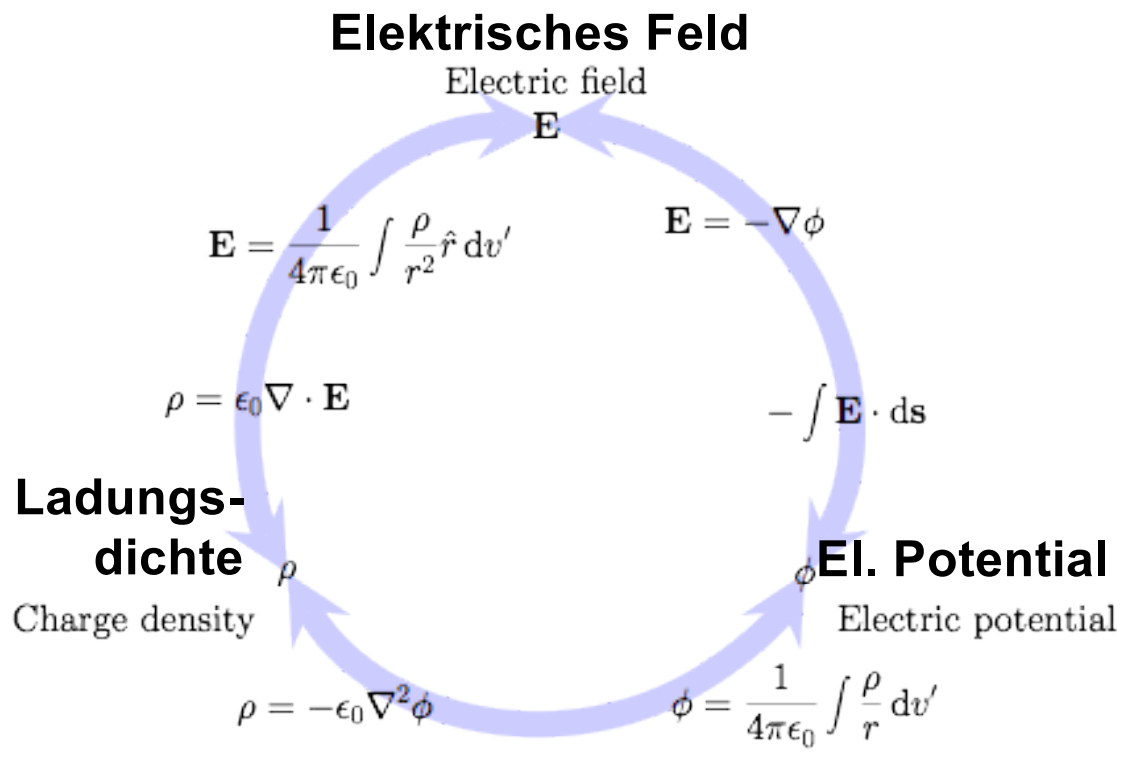
\includegraphics[width=0.4\textwidth]{Figures/Leiter_Isolatoren.png}
\end{center}
